%%% Ne pas modifier jusqu'à la ligne 25
\documentclass[a4paper,12pt]{book}
\usepackage[utf8]{inputenc}
\usepackage[french]{babel}
%%\usepackage{CJK}
\usepackage{yhmath}
\usepackage[left=2cm,right=2cm,top=3cm,bottom=2cm, headheight=1.5cm,headsep=1.5cm]{geometry}
%%\usepackage{CJKutf8}
\usepackage{amsfonts}
\usepackage{amsmath,amsfonts,amssymb,dsfont}
\usepackage{graphicx}
\usepackage{enumitem}		%\enumerate-resume
\usepackage[colorlinks=true,unicode={true},hyperindex=false, linkcolor=blue, urlcolor=blue]{hyperref}
\newcommand{\myref}[1]{\ref{#1} page \pageref{#1}}

\addto\captionsfrench{\def\tablename{Tableau}}  %légendes des tableaux
\renewcommand\thesection{\Roman{section}~-~} 
\renewcommand\thesubsection{\Roman{section}.\Alph{subsection}~-~} 
\renewcommand\thesubsubsection{\Roman{section}.\Alph{subsection}.\arabic{subsubsection}~-~} 

\newcommand{\conclusion}[1]{\newline \centerline{\fbox{#1}}}

\setcounter{secnumdepth}{3}
\parindent=0pt

\usepackage{fancyhdr}
\pagestyle{fancy}

\lhead{SJTU-ParisTech} 
%%%%%%%%%%%%%%%%%%%%%%%%%%%%%%%%%%
\chead{TR3}
\rhead{Daniel 518261910024}

\begin{document}
\renewcommand{\labelitemi}{$\blacktriangleright$}
\renewcommand{\labelitemii}{$\bullet$}


\section{la distance maximale}
\begin{figure}[h]
    \begin{center}
    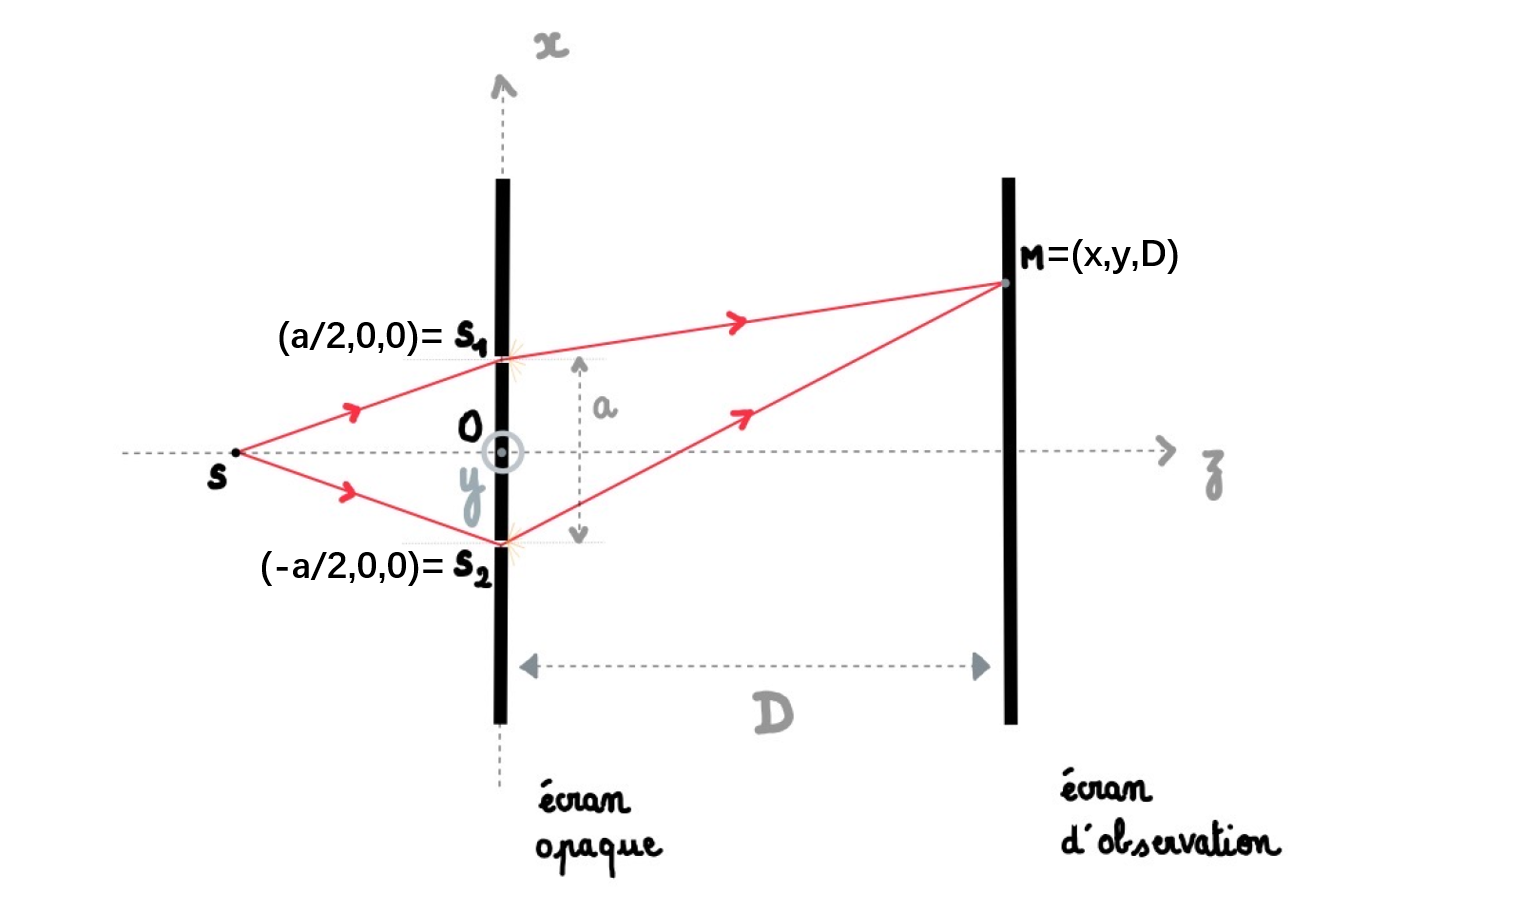
\includegraphics[scale=0.8]{tr2.png}
    \end{center}
    \caption{Expérience des trous de Young}
\end{figure}
Par les résultats précédents, on sait que $i=\frac{\lambda_0D}{a}$ 
par notre hypothèses ($|a| \ll D, |x| \ll D, |y| \ll D$).
On a donc $a=\frac{\lambda_0D}{i}$. Lorsque l’interfrange soit 
d’au moins $i_0=1,0\,mm$, sur un écran placé à une distance égale à $D=2,0\,m$ 
des sources, longueur d'onde $\lambda_0=500\,nm$, observé dans l'air, on a $\boxed{a_0 \leq \frac{\lambda_0D}{i_0}}$, 
avec $a_0$ la distance maximale entre les deux trous. 

A.N. $\boxed{a_0 \leq \frac{500*10^{-9}*2,0}{1,0*10^{-3}}=1,0*10^{-3}m}$. 
On a $|a_0| \ll D $, ce qui satisfait notre hypothèse, 

\end{document}